The aim of this chapter is to introduce \textit{control methods} for \textbf{spacecraft}, then we will include the spacecraft (described by Dynamic-Kinematic equations) in a \textbf{feedback loop}. The \textit{Attitude Control System} is in charge to:
\begin{enumerate}
    \item Give a proper orientation to the body
    \item Stabilize the spacecraft about a reference in the presence of disturbance torques.
\end{enumerate}
\begin{quote}
    \textsf{
        Important: The Attitude orientation is fundamental in any space mission.
    }
\end{quote}

\begin{figure}[h]
    \centering
    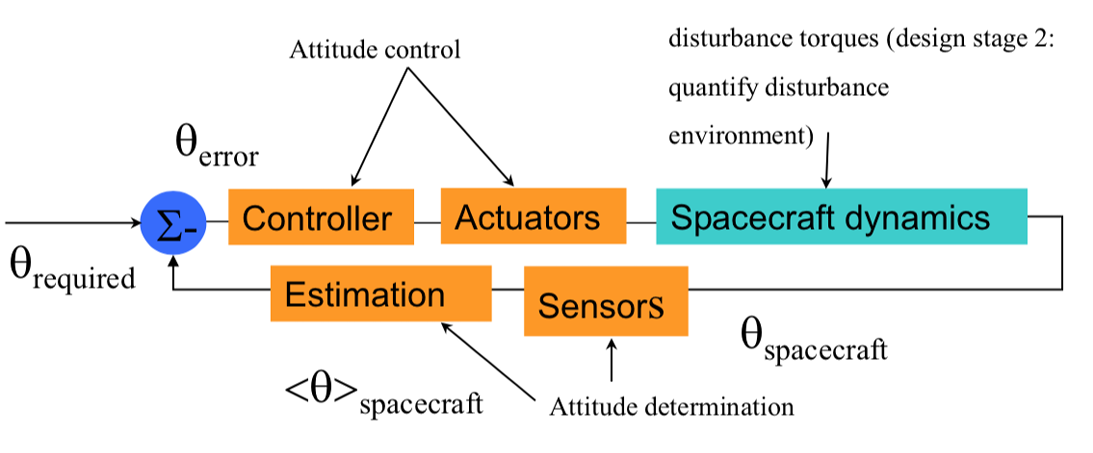
\includegraphics[scale=0.6]{AerospaceApplications/images/ACS.png}
    \caption{Attitude Control System}
\end{figure}

\section{Sensors}
A \textbf{sensor} employed in this field must be able to provide \textbf{in real time} the measurement of the attitude. This is fundamental to build any effective control system. The available sensors can be broken into two families:
\begin{itemize}
    \item \textbf{Absolute attitude sensors} which determine the attitude with respect to some celestial body like the Sun or other stars (an example can be a \textbf{star tracker}).
    \item  \textbf{Relative attitude sensors} they are capable to measure the \textit{angular rate}, then the attitude is obtained through integration (they are usually \textbf{gyroscopes}).
\end{itemize}

\section{Actuators}
An \textbf{actuator} is fundamental in order to give to the system to control (the spacecraft) the \textbf{control input}. Even here three groups of actuators can be distinguished:
\begin{enumerate}
    \item \textbf{Dampers} which are used to reduce the effect of nutation and external disturbances torques;
    \item \textbf{Actuators which provides external torques}, they include \textit{thrusters, reaction wheels, particular types of Gyros};
    \item \textbf{Actuators which use external forces} like magnetic fields, gravity gradient and so on.
\end{enumerate}
The control laws we will present can be applied by using thrusters, reaction wheels or combination of them.

\section{Control system approaches}
How it has been mentioned in the introduction, the main objective of an attitude control system can be the \textbf{stabilization} about a reference attitude, or the tracking in the case that the orientation changes in time.
We can split the \textit{attitude control systems} in three categories:
\begin{enumerate}
    \item \textsc{Passive}: they are based on enviromental forces and on the properties of the body. They exist because environment perturbations can lead to stable behaviours. Passive control systems are seldom used.
    \item \textsc{Semi-active}, in this case some \textit{reaction wheels} are used that exploit the angular momentum consevation. Alternatively can be used \textit{magnetic systems} which interacting with the magnetic field tend to produce useful torques.
    \item \textsc{Active}: is the most used in the field of ACS (Attitude Control Systems), the technique is based on the use of \textit{thrusters}.
\end{enumerate}
\begin{quote}
    \textsf{
        A lot of classifications are available, another possible classification is that beetween: \textit{Spin stabilization} and \textit{3-axis stabilization}. The presented approach is based on \textbf{Three-axis control}.
    }
\end{quote}

\section{Attitude control: a general setting}
In the previous chapter we have seen the equations for dynamics and kinematics of a spacecraft, moreover we have understood that a useful and effective description of the orientation can be provided by  \textit{quaternions}, as they are powerful and \textit{gimbal lock free}.\\
The \textbf{general goal} of \textit{control} is to make the state vector $(\mathfrak{q}, \boldsymbol{\omega})$ track a \textbf{reference vector} $(\mathfrak{q}_r, \boldsymbol{\omega_r})$ which can be eventually time-varying. In order to determine what is the 'distance' from the desired behaviour we have to compute the tracking error:
\begin{itemize}
    \item The \textbf{angular velocity tracking error} is defined simply as
    \begin{equation*}
        \tilde{\boldsymbol{\omega}} \doteq \boldsymbol{\omega}_r - \boldsymbol{\omega}
    \end{equation*}
    \item The \textbf{quaternion tracking error} is defined as a product beetween quaternions
    \begin{equation*}
        \tilde{\mathfrak{q}} \equiv \begin{bmatrix}
          \   \tilde{q_0} \ \\\ \tilde{\mathbf{q}} \
        \end{bmatrix} \doteq \mathfrak{q}^{-1} \otimes \mathfrak{q}_r = \mathfrak{q}^* \otimes \mathfrak{q}_r
    \end{equation*}
    The quaternion $\tilde{\mathfrak{q}}$ is nothing but the quaternion which starting from $\mathfrak{q}$ goes to $\mathfrak{q}_r$. 
\end{itemize}

\section{First problem: Regulation}

\section{Second problem: Tracking}